% !Mode:: "TeX:UTF-8"
%% 请使用 XeLaTeX 编译本文.
% \documentclass{WHUBachelor}% 选项 forprint: 交付打印时添加, 避免彩色链接字迹打印偏淡. 即使用下一行:
\documentclass[forprint]{WHUBachelor}
\usepackage{geometry}
\usepackage{float}
\usepackage{minted}
\usepackage{algorithm}
\usepackage{algorithmicx}
\usepackage{algpseudocode}
\usepackage{amsmath}

\begin{document}
%%%%%%% 下面的内容, 据实填空.

\title{吃豆人程序的设计 \\ {\Large《人工智能导论》实验报告}}
\author{马玉坤}                            % 作者名字
\Cmajor{计算机科学与技术}                  % 专业中文名
\Cschoolname{计算机科学与技术系}          % 学院名
\Csupervisor{李钦策}        %指导教师中文名、职称
\date{二〇一八年一月}                    % 日期, 要注意和英文日期一致!!
\teammates{李伟枫,许浩禹,张宁}
\StudentNumber{1150310618}

%-----------------------------------------------------------------------------
\pdfbookmark[0]{封面}{title}         % 封面页加到 pdf 书签
\maketitle
\frontmatter
\pagenumbering{Roman}              % 正文之前的页码用大写罗马字母编号.
%-----------------------------------------------------------------------------
% !Mode:: "TeX:UTF-8"

%%% 此部分需要自行填写: (1) 中文摘要及关键词 (2) 英文摘要及关键词

%%======中文摘要===========================%
\begin{cnabstract}
  在本次CPU设计过程中,本人在两位实验课老师和Digilent社区的帮助下,设计了一个可在Nexys 4 DDR上运行的,有固定指令周期的且支持十条指令的精简指令集 (RISC) 处理器。本文详细介绍了本人在计算机设计与实践实验课上完成计算机设计与实践实验5的相关设计。本文内容包括: (1) CPU的顶层设计; (2) CPU各个模块,包括取指模块、运算模块、访存模块、回写模块、内存控制以及IO控制若干个模块的内部设计; (3)进行CPU设计及实现过程中遇到的问题与解决方法; (4) Digilent Nexys 4 DDR FPGA的简单介绍。

\end{cnabstract}
\par
\vspace*{2em}


%%%%--  关键词 -----------------------------------------%%%%%%%%
%%%%-- 注意: 每个关键词之间用“;”分开,最后一个关键词不打标点符号
\cnkeywords{中央处理器; CPU; FPGA; VHDL; 计算机设计与实践 }
    % 加入摘要, 申明.
%==========================把目录加入到书签==============================%%%%%%
\pdfbookmark[0]{目录}{toc}
\tableofcontents
\mainmatter %% 以下是正文
%%%%%%%%%%%%%%%%%%%%%%%%%%%--------main matter-------%%%%%%%%%%%%%%%%%%%%%%%%%%%%%%%%%%%%

\chapter{简介}

吃豆人项目\cite{berkeley}是加州大学伯克利分校为入门级人工智能课程开发的项目。通过一系列的AI技术来玩吃豆人。但是吃豆人项目不专注于为视频游戏构建AI,恰恰相反这些项目教授使用者AI基础概念,如知情的状态空间搜索,概率推理和强化学习。这些概念是真实世界的应用领域,如自然语言处理,计算机视觉和机器人。

这些项目允许学生可视化实现的技术的结果。它们还包含代码示例和明确的指示,但不要强迫学生趟过过多的脚手架。最后,吃豆人提供了一个具有挑战性的问题环境,需要创造性的解决方案; 真实世界的AI问题是具有挑战性的,吃豆人也是。

吃豆人系列项目一共分为五个小项目:Search, Multiagent Search, Reinforcement Learning, Ghostbusters以及Classification。其中的项目一——Search就是我们本次的实验。在这个实验中,吃豆人将通过一系列构建的一系列的搜索算法实现达到特定位置并有效地吃到食物。包括深度优先搜索、广度优先搜索、一致代价搜索、A*搜索、启发式搜索等8个问题。

这八个问题分别是:

\begin{enumerate}
\item 应用深度优先算法找到一个特定的位置的豆
\item 宽度优先算法
\item 代价一致算法
\item A* 算法
\item 找到所有的角落
\item 角落问题(启发式)
\item 吃掉所有的豆子
\item 次最优搜索
\end{enumerate}

在这个实验的实现过程中需要编辑两个关键文件“search.py”和“searchAgents.py”,“search.py”中需要补充编写四个基本搜索算法,“searchAgents.py”中需要补充编写所有启发式算法的基本内容。除此之外还有三个比较重要的文件:“pacman.py”、“game.py”和“util.py”。“pacman.py”是游戏的主文件,描述了一个Pacman GameState类型。“game.py”说明了Pacman世界如何工作的逻辑并且描述了几种支持类型,如AgentState,Agent,Direction和Grid。“util.py”是对我们来说非常重要的文件,包括了实现搜索算法可以用到的几种数据结构。

通过这个实验,我们可以更好的理解各种基本搜索算法,并且通过可视化的方法可以更加有成就感,激发学习兴趣。在人工智能的领域继续研究下去。

\chapter{算法介绍}

\section{编写通用搜索算法}

\subsection{待解决问题的解释}

编写一个通用的搜索算法,来解决“应用深度优先算法找到一个特定的位置的豆”,“应用深度优先算法找到一个特定的位置的豆”,“应用深度优先算法找到一个特定的位置的豆”,“应用深度优先算法找到一个特定的位置的豆”等四个问题。

\subsection{问题的形式化描述}

\textbf{输入:}problem(吃豆人游戏搜索问题),open(遍历所用的数据结构),heurisitic(启发式算法)

\textbf{输出:}path[](由方向组成的数组,可以指示吃豆人从起始状态走到终止状态)

\subsection{解决方案介绍}

四种算法既有相似性也有相异性。相似性体现在四种算法的框架类似,相异性主要体现在两个方面。

第一个方面便是启发式函数的问题。在四个问题中,最复杂的问题是A*搜索问题,因为A*搜索问题需要启发式函数。换个角度来看,其他三种算法(深度优先搜索,广度优先搜索以及代价一致搜索)可以看做是启发式函数恒为0。

第二个方面数据结构的不同。

因此四种问题只需分别定义好数据结构以及启发函数,调用通用搜索算法便可以获得解决方案。

\subsection{所用方法的一般介绍}

我们定义了一个函数unifiedSearch(意为通用搜索),unifiedSearch需要三个参数,首先是搜索问题,第二个是遍历所用的数据结构对象,最后一个是所用的启发式(估价)函数。

函数执行的第一步便是初始化过程,将初始状态的$f,g,h$($f[state]=g[state]+h[state]$,其中$h$为启发式函数)三个函数定义好,然后将初始状态push到数据结构对象中。

接下来便是遍历过程,每次从数据结构对象中pop元素,设为当前的状态,然后判断当前状态是否为结束状态,如果是结束状态就返回找到的路径,否则就扩展新的状态,放到数据结构对象中。每次扩展子状态都需要使用启发式函数计算状态的$f[childState]$函数值。

\subsection{算法伪代码}

\floatname{algorithm}{算法}
\renewcommand{\algorithmicrequire}{\textbf{输入:}}
\renewcommand{\algorithmicensure}{\textbf{输出:}}
\begin{algorithm}[H]
  \caption{通用搜索算法}
  \begin{algorithmic}[1] %每行显示行号
    \Require $problem$搜索问题,$open$遍历所需的数据结构对象,$heuristic$启发式函数
    \Ensure 指示从起点到终点的路径的方向列表
    \State $initialState \gets problem.getStartstate()$
    \State 初始化$initialState$的$f,g,h$函数
    \State $open.push(initialState)$
    \While {$open$非空}
    \State $state \gets open.pop()$
    \State 将$state$加入$close$表
    \If {$state$为结束状态}
    \State \Return{\Call{getPath}{$state, initialState$}}
    \EndIf
    \For {$childState$ in $state$的子状态}
    \State 更新$childState$的信息
    \State 将$childState$加入$open$
    \EndFor
    \EndWhile

    \Function {getPath}{$dest, src$}
    \State $state \gets dest$
    \State $path \gets []$
    \While {$state \neq src$}
    \State $path \gets path + state$ 的转移方向
    \State $state \gets $ 父状态
    \EndWhile
    \State \Return{$path$}
    \EndFunction
  \end{algorithmic}
\end{algorithm}

\section{找到所有的角落}

\subsection{待解决问题的解释}

需要重新定义问题状态,使状态能够表示四个角落的访问状态,使得该问题使用之前的搜索算法解决时,能够遍历所有的角落(左上、左下、右上、右下四个角落)。

\subsection{问题的形式化描述}

修改searchAgents.py文件中的CornersProblem类。编写$\_\_init\_\_()$、$getStartState()$、$isGoalState()$以及$getSuccessors()$方法,使得CornersProblem能够成为一个自洽的问题,且当问题解决时,四个角落都会被访问到。

\subsection{解决方案介绍}

其实,定义好这样一个问题,只需要考虑清楚如何将四个角落的访问状态加入到状态中。因此我们在状态设计中新增维数,添加表示角落访问状态的维度,从而来表示状态。

\subsection{所用方法的一般介绍}

在之前的问题中,状态的表示为一个二元组$(x,y)$。在该问题中,我们设计了一个新的维度,用来存储四个角落的访问状态。新的状态形式为$((x,y),corners)$,是一个新的二元组,该二元组的第一维是一个坐标二元组,第二维是一个4位二进制数$corners$。

当$corners$为$1111$时,表示四个角落都访问过,这也是终止状态的充分必要条件。当$corners$为$1000$时,表示仅仅访问过左上角落。而当$corners$为$0000$时,表示四个状态都没有访问过。初始状态即为$(startingPosition, 0000)$。

\subsection{算法伪代码}


\begin{algorithm}[H]
  \caption{角落问题}
  \begin{algorithmic}[1] %每行显示行号
    \Function {getStartState} {$self$}
    \State \Return {$(self.startingPosition, 0)$}
    \EndFunction

    \Function {isGoalState} {$self, state$}
    \If {$state[1] = 15$}
    \State \Return {True}
    \Else
    \State \Return {False}
    \EndIf
    \EndFunction

    \Function {getSuccessors} {$self, state$}
    \State $successors \gets []$
    \For {$action \in Directions$}
    \State 从action和当前位置获取新的位置
    \State 从新位置和当前四个角落的访问情况获取新的四个角落的访问情况
    \If {新位置可达}
    \State $successors \gets successors + $新状态
    \EndIf
    \EndFor
    \State \Return{$successors$}
    \EndFunction
  \end{algorithmic}
\end{algorithm}

\section{角落问题(启发式)}

\subsection{待解决问题的解释}

编写上一个问题(角落问题)对应的A*算法的启发式函数。

\subsection{问题的形式化描述}

\textbf{输入:}当前状态$state$,当前问题$problem$

\textbf{输出:}当前状态对应的估价函数值

\subsection{解决方案介绍}

枚举访问顺序,通过曼哈顿距离测算最小的代价。

\subsection{所用方法的一般介绍}

由于没有访问的角落最多只有四个,所以我们可以枚举四个角落的访问顺序(最多$4!=24$种),找到代价最小的访问顺序,代价的计算是通过曼哈顿距离来测算的,这样效率比较高,拿到了满分。

\subsection{算法伪代码}

\begin{algorithm}[H]
  \caption{角落问题启发式函数}
  \begin{algorithmic}[1] %每行显示行号
    \Require $state$当前状态,$problem$搜索问题
    \Ensure 当前状态的启发式函数值
    \State $minDist \gets \infty$
    \For {$perm \in [0,1,2,3]$的四种排列}
    \State $dist \gets $使用曼哈顿距离计算的按照排列顺序所需的最小代价
    \State $minDist \gets min(minDist, dist)$
    \EndFor
    \State \Return{$minDist$}
  \end{algorithmic}
\end{algorithm}

\section{吃掉所有的豆子}

\subsection{待解决问题的解释}

编写\emph{searchAgents.py}中的$foodHeuristic$函数,能够成为使用A*算法解决$FoodSearchProblem$的启发式函数。

\subsection{问题的形式化描述}

补充\emph{searchAgents.py}中的$foodHeuristic$函数,使得其是一个consistent且admissible的启发函数。

\textbf{输入:}当前状态$state$,当前吃掉所有豆子的问题$problem$

\textbf{输出:}一个数字,表示当前状态的估价函数值

\subsection{解决方案介绍}

在吃掉所有豆子的问题中,状态的定义为$((x,y), foodList)$。$foodList$表示所有豆子的位置列表。当豆子列表为空时,显然估计函数值应该为0。当豆子列表不为空的时候,我们只需要计算所有豆子中,与当前位置曼哈顿距离最大的豆子,距离当前位置的精确距离(使用\emph{searchAgents.py}中的$mazeDistance$)就能达到非常惊人的效果,获得了5/4的分数。

\subsection{所用方法的一般介绍}

当豆子列表为空时,显然估计函数值应该为0。当豆子列表不为空的时候,我们只需要计算所有豆子中,与当前位置曼哈顿距离最大的豆子,距离当前位置的精确距离(使用\emph{searchAgents.py}中的$mazeDistance$)。

\subsection{算法伪代码}

\begin{algorithm}[H]
  \caption{吃掉所有豆子的启发式函数}
  \begin{algorithmic}[1] %每行显示行号
    \Require $state$当前状态,$problem$搜索问题
    \Ensure 当前状态的启发式函数值
    \State $position \gets $当前状态的位置
    \State $foodList \gets $当前状态中所有没吃掉的豆子的位置列表
    \If {$|foodList| = 0$}
    \State \Return{$0$}
    \Else
    \State $farestFood \gets foodList$中距离$position$最近的豆子的位置
    \State \Return{$farestFood$ 距离 $position$的精确位置($mazeDistance$)}
    \EndIf
  \end{algorithmic}
\end{algorithm}

\section{次最优搜索}

\subsection{待解决问题的解释}

定义一个优先吃最近的豆子函数是提高搜索速度的一个好的办法。补充完成searchAgents.py文件中的AnyFoodSearchProblem目标测试函数,并完成searchAgents.py文件中的ClosestDotSearchAgent部分,在此Agent当中缺少一个关键的函数:找到最近豆子的函数。

\subsection{问题的形式化描述}

补充\emph{searchAgents.py}中的$ClosetDotSearchAgent$类中的$findPathToClosetDot$函数。

\textbf{输入:}gameState游戏状态

\textbf{输出:}一条路径,能够从当前位置走到最近的豆子的位置

\subsection{解决方案介绍}

使用之前定义的$bfs$函数,来解决这个问题即可。

\subsection{所用方法的一般介绍}

使用$search.bfs(problem)$可以调用之前写好的bfs函数,返回值即为当前位置到最近的豆子的位置的路径。

\subsection{算法伪代码}

\begin{algorithm}[H]
  \caption{找到到最近的豆子的路径}
  \begin{algorithmic}[1] %每行显示行号
    \Require $gameState$游戏状态
    \Ensure 从当前吃豆人的位置到最近的豆子的路径
    \State $problem \gets $ \Call{AnyFoodSearchProblem} {$gameState$}
    \State $path \gets $ \Call{bfs} {$problem$}
    \State \Return{$path$}
  \end{algorithmic}
\end{algorithm}

\chapter{算法实现}

\section{实验环境}

\textbf{实验环境:}

\begin{itemize}
\item CPU:E3-1230 v5
\item 操作系统:Arch Linux
\item 内核版本:Linux version 4.14.11-1-ARCH
\end{itemize}

\section{数据结构}

本实验使用了多种数据结构,包括:

\begin{enumerate}
\item 栈
\item 队列
\item 优先队列
\item 字典(哈希表)
\item 列表(线性表)
\end{enumerate}

\section{实验结果}

实验证明,最终我们使用的方法非常出色,得到了26/25的总分数(满分25,在问题7中得到了1分加分)。

\section{系统中间及最终输出结果}

\begin{figure}[H]
  \centering
  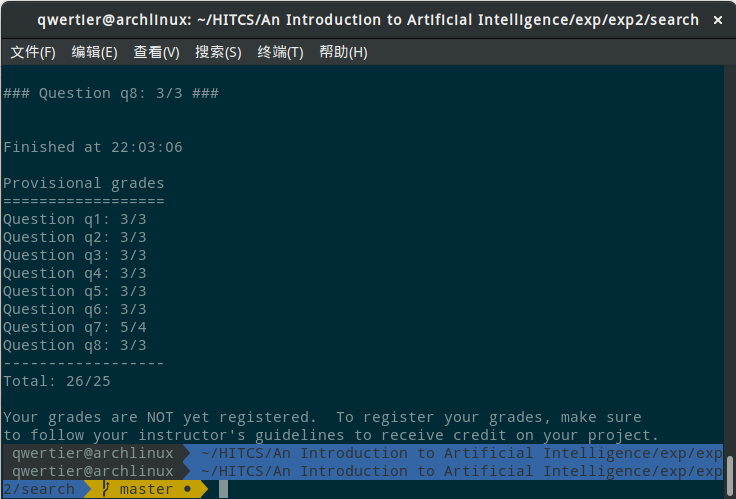
\includegraphics[width=6in]{figures/result.png}
  \caption{结果截图}\label{fig:result}
\end{figure}

\chapter{总结及讨论}

在本次实验的8个问题中,我们明确分工,积极讨论,认真研读课上讲义,广泛查阅资料\cite{AI}。整个实验的难度并不高,因此我们完成得较为迅速。最终的成果令我们十分开心。

令人印象深刻的是在问题7(评分标准如图\ref{fig:problem7})中,当我们在猜想,实验,推倒,再猜想,再实验,再推倒的过程中,一系列启发式函数要么效果不佳(只能得部分分数),要么不满足可纳性,要么不满足一致性。当我们进行了很多次尝试之后,终于找到了现在这个效果好,且满足两个性质的启发式函数。

\begin{figure}[H]
  \centering
  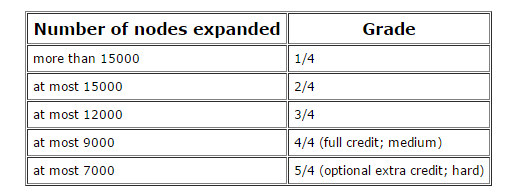
\includegraphics[width=6in]{figures/problem7.png}
  \caption{问题7的评分标准}\label{fig:problem7}
\end{figure}

完成该实验之后,经过反思,我们首先认为这个实验过程十分有趣,通过补充编写吃豆人这个游戏,来学习人工智能导论的基础知识。加州伯克利分校\cite{berkeley}的这种寓教于乐的方式很值得我们学习。其次,我们对人工智能导论的学习也产生了更浓厚的兴趣,在接下来的时间中,我们会更认真学习人工智能导论课程的知识。

%%%=== 参考文献 ========%%%
\cleardoublepage\phantomsection
\addcontentsline{toc}{chapter}{参考文献}
%\bibliographystyle{agsm}
\bibliography{ref}

%%% !Mode:: "TeX:UTF-8"
%%%%%%%%%%%%%%%%%%%%%%%%%%%%-------致谢--------%%%%%%%%%%%%%%%%%%%%%%%%%%%%%%%%

\acknowledgement
\addcontentsline{toc}{chapter}{致谢}

感谢罗丹彦老师和助教学长的耐心指导,实验5的完成离不开他们的指点。











 %%%致谢

%%%-------------- 附录. 不需要可以删除.-----------

\appendix

\chapter{实验代码}

\section{通用搜索算法}

\begin{minted}[fontsize=\small]{Python}
def unifiedSearch(problem, open, heuristic):
    closed = set()
    preDirection = dict()
    prePosition = dict()
    f = dict()
    g = dict()
    h = dict()

    def getPath(dest, src):
        # 获得从起点(src)到终点(dest)的路径,由dest向前遍历得到
        state = dest
        path = []
        while state != src:
            path.append(preDirection[state])
            state = prePosition[state]
        path.reverse()
        return path

    initialState = problem.getStartState()
    g[initialState] = 0
    h[initialState] = heuristic(initialState, problem)
    f[initialState] = g[initialState] + h[initialState]
    open.push((initialState, f[initialState], None, None))

    while not open.isEmpty():
        (state, _, prePositionTmp, preDirectionTmp) = open.pop()
        if state in closed:
            continue
        preDirection[state] = preDirectionTmp  # 找到从父状态所转移来的方向
        prePosition[state] = prePositionTmp  # 找到父状态
        closed.add(state)
        if problem.isGoalState(state):  # 到达终点
            return getPath(state, problem.getStartState())
        for childState in problem.getSuccessors(state):
            if childState[0] not in g:  # 子状态的g函数未定义
                g[childState[0]] = g[state] + childState[2]
            else:
                g[childState[0]] = min(g[childState[0]], g[state] + childState[2])
            if childState[0] not in h:  # 子状态的h函数未定义
                h[childState[0]] = heuristic(childState[0], problem)
            if childState[0] not in f:
                f[childState[0]] = g[childState[0]] + h[childState[0]]
            else:
                f[childState[0]] = min(f[childState[0]], g[childState[0]] +
                                                         h[childState[0]])
            open.push((childState[0], f[childState[0]], state, childState[1]))
    return []

def depthFirstSearch(problem):
    """
    Search the deepest nodes in the search tree first.

    Your search algorithm needs to return a list of actions that reaches the
    goal. Make sure to implement a graph search algorithm.

    To get started, you might want to try some of these simple commands to
    understand the search problem that is being passed in:
    print "Start:", problem.getStartState()
    print "Is the start a goal?", problem.isGoalState(problem.getStartState())
    print "Start's successors:", problem.getSuccessors(problem.getStartState())
    """
    return unifiedSearch(problem, util.Stack(), nullHeuristic)
    return []

def breadthFirstSearch(problem):
    """Search the shallowest nodes in the search tree first."""
    return unifiedSearch(problem, util.Queue(), nullHeuristic)

def uniformCostSearch(problem):
    """Search the node of least total cost first."""
    return unifiedSearch(problem, util.PriorityQueueWithFunction(lambda x: x[1]),
                         nullHeuristic)

def nullHeuristic(state, problem=None):
    """
    A heuristic function estimates the cost from the current state to the nearest
    goal in the provided SearchProblem.  This heuristic is trivial.
    """
    return 0

def aStarSearch(problem, heuristic=nullHeuristic):
    """Search the node that has the lowest combined cost and heuristic first."""
    return unifiedSearch(problem, util.PriorityQueueWithFunction(lambda x: x[1]),
                         heuristic)


# Abbreviations
bfs = breadthFirstSearch
dfs = depthFirstSearch
astar = aStarSearch
ucs = uniformCostSearch
\end{minted}

\section{角落问题}

\begin{minted}[fontsize=\small]{Python}

class CornersProblem(search.SearchProblem):
    """
    This search problem finds paths through all four corners of a layout.

    You must select a suitable state space and successor function
    """

    def __init__(self, startingGameState):
        """
        Stores the walls, pacman's starting position and corners.
        """
        self.walls = startingGameState.getWalls()
        self.startingPosition = startingGameState.getPacmanPosition()
        top, right = self.walls.height-2, self.walls.width-2
        self.corners = ((1,1), (1,top), (right, 1), (right, top))
        for corner in self.corners:
            if not startingGameState.hasFood(*corner):
                print 'Warning: no food in corner ' + str(corner)
        self._expanded = 0 # DO NOT CHANGE; Number of search nodes expanded
        # Please add any code here which you would like to use
        # in initializing the problem

    def getStartState(self):
        """
        Returns the start state (in your state space, not the full Pacman state
        space)
        """
        "*** YOUR CODE HERE ***"
        return (self.startingPosition, 0)

    def isGoalState(self, state):
        """
        Returns whether this search state is a goal state of the problem.
        """
        "*** YOUR CODE HERE ***"
        if state[1] == 15:
            return True
        else:
            return False

    def getSuccessors(self, state):
        """
        Returns successor states, the actions they require, and a cost of 1.

         As noted in search.py:
            For a given state, this should return a list of triples, (successor,
            action, stepCost), where 'successor' is a successor to the current
            state, 'action' is the action required to get there, and 'stepCost'
            is the incremental cost of expanding to that successor
        """

        successors = []
        for action in [Directions.NORTH, Directions.SOUTH, Directions.EAST, Directions.WEST]:
            # Add a successor state to the successor list if the action is legal
            # Here's a code snippet for figuring out whether a new position hits a wall:
            #   x,y = currentPosition
            #   dx, dy = Actions.directionToVector(action)
            #   nextx, nexty = int(x + dx), int(y + dy)
            #   hitsWall = self.walls[nextx][nexty]

            "*** YOUR CODE HERE ***"
            x,y = state[0]
            dx, dy = Actions.directionToVector(action)
            nextx, nexty = int(x + dx), int(y + dy)
            hitsWall = self.walls[nextx][nexty]

            # 获得新的二进制数,表示四个角落的访问状态
            isCorner = 0
            for i in xrange(len(self.corners)):
                corner = self.corners[i]
                if (nextx, nexty) == corner:
                    isCorner |= 1 << i

            if not hitsWall: # 没有撞墙
                successors.append((((nextx,nexty), state[1]|isCorner), action, 1))

        self._expanded += 1 # DO NOT CHANGE
        return successors

    def getCostOfActions(self, actions):
        """
        Returns the cost of a particular sequence of actions.  If those actions
        include an illegal move, return 999999.  This is implemented for you.
        """
        if actions == None: return 999999
        x,y= self.startingPosition
        for action in actions:
            dx, dy = Actions.directionToVector(action)
            x, y = int(x + dx), int(y + dy)
            if self.walls[x][y]: return 999999
        return len(actions)

\end{minted}

\section{角落问题(启发式)}

\begin{minted}[fontsize=\small]{Python}

import itertools
def cornersHeuristic(state, problem):
    """
    A heuristic for the CornersProblem that you defined.

      state:   The current search state
               (a data structure you chose in your search problem)

      problem: The CornersProblem instance for this layout.

    This function should always return a number that is a lower bound on the
    shortest path from the state to a goal of the problem; i.e.  it should be
    admissible (as well as consistent).
    """
    corners = problem.corners # These are the corner coordinates
    walls = problem.walls # These are the walls of the maze, as a Grid (game.py)

    "*** YOUR CODE HERE ***"
    def manhattan(p1, p2):
        return abs(p1[0]-p2[0]) + abs(p1[1]-p2[1])
    minDist = -1
    cornerState = state[1]

    # 枚举4!=24中排列
    for perm in itertools.permutations([0,1,2,3], 4):
        dist = 0
        lastPos = state[0]

        # 计算按顺序遍历这四个角落需要的最少步数
        for i in perm:
            if ((cornerState >> i) & 1) == 0:
                dist += manhattan(corners[i], lastPos)
                lastPos = corners[i]
                #print corners, perm, cornerState, dist
        if minDist == -1:
            minDist = dist
        else:
            minDist = min(minDist, dist)
    return max(minDist, 0) # Default to trivial solution

\end{minted}

\section{吃掉所有的豆子}

\begin{minted}[fontsize=\small]{Python}

def foodHeuristic(state, problem):
    """
    Your heuristic for the FoodSearchProblem goes here.

    This heuristic must be consistent to ensure correctness.  First, try to come
    up with an admissible heuristic; almost all admissible heuristics will be
    consistent as well.

    If using A* ever finds a solution that is worse uniform cost search finds,
    your heuristic is *not* consistent, and probably not admissible!  On the
    other hand, inadmissible or inconsistent heuristics may find optimal
    solutions, so be careful.

    The state is a tuple ( pacmanPosition, foodGrid ) where foodGrid is a Grid
    (see game.py) of either True or False. You can call foodGrid.asList() to get
    a list of food coordinates instead.

    If you want access to info like walls, capsules, etc., you can query the
    problem.  For example, problem.walls gives you a Grid of where the walls
    are.

    If you want to *store* information to be reused in other calls to the
    heuristic, there is a dictionary called problem.heuristicInfo that you can
    use. For example, if you only want to count the walls once and store that
    value, try: problem.heuristicInfo['wallCount'] = problem.walls.count()
    Subsequent calls to this heuristic can access
    problem.heuristicInfo['wallCount']
    """
    position, foodGrid = state
    "*** YOUR CODE HERE ***"

    def manhattan(p1, p2):
        return abs(p1[0]-p2[0])+abs(p1[1]-p2[1])
    foodList = foodGrid.asList()

    if len(foodList) == 0:
        return 0
    else:
        # 找到曼哈顿距离最近的
        farest = max([(manhattan(food, position), food) for food in foodList])
        # 然后返回准确的最短距离
        return mazeDistance(position, farest[1], problem.startingGameState)

\end{minted}

\section{次最优搜索}

\begin{minted}[fontsize=\small]{Python}

class ClosestDotSearchAgent(SearchAgent):
    "Search for all food using a sequence of searches"
    def registerInitialState(self, state):
        self.actions = []
        currentState = state
        while(currentState.getFood().count() > 0):
            nextPathSegment = self.findPathToClosestDot(currentState) # The missing piece
            self.actions += nextPathSegment
            for action in nextPathSegment:
                legal = currentState.getLegalActions()
                if action not in legal:
                    t = (str(action), str(currentState))
                    raise Exception, 'findPathToClosestDot returned an illegal move: %s!\n%s' % t
                currentState = currentState.generateSuccessor(0, action)
        self.actionIndex = 0
        print 'Path found with cost %d.' % len(self.actions)

    def findPathToClosestDot(self, gameState):
        """
        Returns a path (a list of actions) to the closest dot, starting from
        gameState.
        """
        # Here are some useful elements of the startState
        startPosition = gameState.getPacmanPosition()
        food = gameState.getFood()
        walls = gameState.getWalls()
        problem = AnyFoodSearchProblem(gameState)

        "*** YOUR CODE HERE ***"
        path = search.bfs(problem)
        return path

\end{minted}

\cleardoublepage

\end{document}
